\chapter[Идентификация линейных стохастических систем второго типа]{%
  ИДЕНТИФИКАЦИЯ ЛИНЕЙНЫХ СТОХАСТИЧЕСКИХ СИСТЕМ
}

Как отмечалось в разделе~\ref{ssec:state_criterion},
{\color{red}
  задача линейной аппроксимации полустохастического объекта полностью решена в
  рамках классического линейного регрессионного анализа как задача оценивания параметров
  линейной математической модели объекта с критерием минимизации суммы квадратов вертикальных расстояний.
  Оптимальное решение здесь "--- классическая линейная регрессия,
  обеспечивающая как оптимальное оценивание параметров математической модели объекта
  (при заданных значениях входных переменных),
  так и оптимальное прогнозирование наблюдений выходных переменных по наблюдениям входных переменных.

  Ввиду того, что стохастический объект первого типа не имеет реальных параметров,
  сравнение точности оценивания его параметров лишено смысла.
  В работах~\cite{mukha_2010, mukha_2011} была сформулирована задача оптимального прогнозирования
  выходных переменных линейного стохастического объекта первого типа и показано,
  что оптимальным линейным предиктором также является классическая линейная регрессия.

  Относительно стохастического объекта второго типа следует отметить,
  что области предпочтительного использования классического и симметричного критериев
  определены недостаточно четко.
}
Поэтому будет рассматриваться вопрос идентификации стохастической системы второго типа.

\section{Математическая модель идентифицируемой системы}

Для обеспечения наглядности сравнения будем рассматривать случай
идентификации линейной скалярной системы.
В этом случае функция регрессии имеет простой вид:
\begin{equation}
  \psi = \alpha + \beta \xi,
  \label{eq:linear_fun_scalar}
\end{equation}
где \( \alpha, \beta \) "--- постоянная составляющая и коэффициент усиления "---
параметры системы. Модель задачи идентификации выглядит следующим образом:
\begin{equation}
  \label{eq:linear_model_scalar}
  \begin{aligned}
  h &= \alpha + \beta \xi, \\
  x &= \xi + \varepsilon_x, \\
  y &= h + \varepsilon_y,
  \end{aligned}
\end{equation}
где \( \xi, h \) "--- фактические значения входной и выходной переменной, \\
\hspace*{6mm} \( \alpha, \beta \) "--- фактические значения параметров объекта, \\
\hspace*{6mm} \( x, y \) "--- наблюдаемые значения входной и выходной переменной, \\
\hspace*{5mm} \( \varepsilon_x, \varepsilon_y \) "--- независимые ошибки измерений значений
входной и выходной переменной, распределенные по нормальному закону:
\(
\varepsilon_x = N(0, \sigma_{\varepsilon_x}),
\varepsilon_y = N(0, \sigma_{\varepsilon_y})
\).

Данная модель была использована для генерации наблюдений входа и выхода системы,
на основании которых были получены оценки её параметров методами на основе
классического и симметричного критериев аппроксимации.
Значения \( \xi_i \) выбирались из равномерного в \( [0, 10] \) распределения.
Для получения каждой оценки \( \hat{\alpha}, \hat{\beta} \) использовались результаты
ста наблюдений \( ( x_i, y_i ), i = \overline{1, n}, n = 100 \).

\section{Методы и алгоритмы идентификации}

\subsection{Классический метод наименьших квадратов}

Классический метод наименьших квадратов ставит своей целью минимизировать сумму
вертикальных расстояний от аппроксимирующей гиперплоскости до результатов наблюдений.
Это соответствует использованию классического критерия идентификации
(рисунок~\ref{fig:state_criteria_classic}):
\begin{equation*}
  \rho_{\text{к}} = \sum_i \rho_{\text{к}_i} \rightarrow \min.
\end{equation*}

Пусть \( \overline{y} \) "--- вектор-столбец наблюдений выходной переменной \( \eta \),
а \( X \) "--- \( (r \times n) \)-матрица измерений вектора \( \overline{\xi} \)
(\( r \) строк матрицы представляют собой векторы значений входных переменных в данном наблюдении,
а \( n \) столбцов "--- векторы значений данной входной переменной во всех наблюдениях).

Алгоритм получения МНК-оценок параметров линейной скалярно-векторной функции регрессии сводится
к вычислению значения вектора~\cite{wiki_lse}
\begin{equation*}
  \hat{\overline{\theta}} = (X^{T}X)^{-1}X^{T} \overline{y}.
\end{equation*}

Выполнение этого алгоритма требует времени, линейно зависящего от числа измерений \( O(n) \),
при выполнении реалистичного условия \( n \gg r \).

\vspace{2\baselineskip}
\subsection{Метод симметричной аппроксимации}

Метод симметричной аппроксимации минимизирует сумму перпендикулярных расстояний
от аппроксимирующей гиперплоскости до результатов наблюдений.
Это соответствует использованию симметричного критерия идентификации
(рисунок~\ref{fig:state_criteria_symmetric}):
\begin{equation*}
  \rho_{\text{с}} = \sum_i \rho_{\text{с}_i} \rightarrow \min.
\end{equation*}

Пусть \( X \) "--- \( (m \times n) \)-матрица измерений.
Первые \( r \) и последние \( m - r \) строк этой матрицы представляют собой векторы наблюдений
входных и выходных переменных соответственно,
а столбцы соответствуют векторам \( \overline{x}_i \) значений переменных в данном наблюдении.

Алгоритм расчета оценок параметров линейной функции регрессии
методом симметричной аппроксимации выглядит следующим образом~\cite{mukha_2016}:
\begin{enumerate}
\item Рассчитываются выборочные моменты случайного вектора наблюдений входных и выходных переменных:
  \begin{equation*}
    \hat{\overline{a}} = \dfrac{1}{n} \sum_{i=1}^n \overline{x}_i, \quad
    \hat{D} =
    \dfrac{1}{n}  \sum_{i=1}^n
    (\overline{x}_i - \hat{\overline{a}})
    (\overline{x}_i - \hat{\overline{a}})^T.
  \end{equation*}
\item Формируется матрица \( P \), состоящая из собственных векторов матрицы \( \hat{D} \),
  расположенных в порядке убывания соответствующих им собственных чисел.
  Формируются матрица \( C \), состоящая из \( r \) первых столбцов матрицы \( P \).
\item Выполняется разбиение матриц \( C \), \( X \) и вектора \( \hat{\overline{a}} \) на блоки:
  \begin{equation*}
    C =
    \begin{pmatrix}
      C_r \\
      C_{m-r}
    \end{pmatrix}, \quad
    X =
    \begin{pmatrix}
      X_r \\
      X_{m-r}
    \end{pmatrix}, \quad
    \hat{\overline{a}} =
    \begin{pmatrix}
      \hat{\overline{a}}_r \\
      \hat{\overline{a}}_{m-r}
    \end{pmatrix}.
  \end{equation*}
  Таким образом, матрицы \( C_r \) и \( X_r \) содержат первые \( r \) строк матриц
  \( C \) и \( X \) соответственно,
  а \( C_{m-r} \) и \( X_{m-r} \) "--- последние \( m - r \) строк этих матриц.
  Вектор \( \hat{\overline{a}}_r \) содержит первые \( r \),
  а \( \hat{\overline{a}}_{m-r} \) "--- последние \( m - r \) элементов вектора
  \( \hat{\overline{a}} \).
\item Рассчитываются значения оценок параметров зависимости~\eqref{eq:linear_fun_scalar}:
  \begin{equation*}
    \begin{aligned}
      \hat{\beta} &= C_{m-r} (C_r)^{-1}, \\
      \hat{\alpha} &= \hat{\overline{a}}_{m-r} - \hat{\beta} \; \hat{\overline{a}}_r.
    \end{aligned}
  \end{equation*}
\end{enumerate}

Подобно МНК, вычислительная сложность этого алгоритма также составляет \( O(n) \),
считая \( n \gg m \).

\subsection{Программная реализация алгоритмов}



\section{Численный анализ точности методов идентификации}

\subsection{Точность оценивания параметров}

Было выполнено сравнение точности оценивания параметров
\( \hat{\alpha}, \hat{\beta} \) системы~\eqref{eq:linear_model_scalar},
полученных классической линейной регрессией и методом симметричной аппроксимации,
в зависимости от c.~к.~о. ошибок наблюдений \( \sigma_{\varepsilon_x}, \sigma_{\varepsilon_y} \).

В качестве величины, характеризующей сравнительную точность оценивания параметров,
использовалась разность средних Евклидовых расстояний
между точными значениями параметров модели и их оценками,
полученными методом наименьших квадратов и методом симметриченой аппроксимации:
\begin{equation*}
  \begin{aligned}
    d &= d_{\text{МНК}} - d_{\text{МСА}}, \\
    d_{\text{МНК}} &= \frac{1}{k} \sum_{j=1}^k \sqrt{(\hat{\alpha}_{\text{МНК}_j} - \alpha)^2 + (\hat{\beta}_{\text{МНК}_j} - \beta)^2}, \\
    d_{\text{МСА}} &= \frac{1}{k} \sum_{j=1}^k \sqrt{(\hat{\alpha}_{\text{МСА}_j} - \alpha)^2 + (\hat{\beta}_{\text{МСА}_j} - \beta)^2},
  \end{aligned}
\end{equation*}
где \( k \) "--- число оценок.

{\color{red}
Таким образом, при \( d > 0 \) точность оценивания параметров модели с помощью МСА
превосходит точность МНК, а при \( d < 0 \) МНК-оценки являются более точными.
При \( d = 0 \) оба метода дают оценки одинаковой точности.
}

Расчеты величины \( d \) производились в узлах сетки значений
\( \sigma_{\varepsilon_x}, \sigma_{\varepsilon_y} \) в прямоугольнике
\( [0, 2] \times [0, 2] \) с шагом 0{,}1.
В каждом узле сетки вычислялось сто оценок (\( k = 100 \)).

На рисунке~\ref{fig:comparison_linear_params_beta-small}
представлены линии равного уровня зависимости \( d(\sigma_{\varepsilon_x}, \sigma_{\varepsilon_y}) \)
при малых значениях коэффициента усиления модели \( \beta \).
Ввиду того, что при \( \sigma_{\varepsilon_y} > \sigma_{\varepsilon_x} \)
значение величины \( d \) невелико по модулю и отрицательно (\( d \in ( -0{,}5, 0 ] \)),
можно сделать вывод, что МНК дает немного более точные оценки параметров, чем МСА.
Поскольку при \( \sigma_{\varepsilon_y} \le \sigma_{\varepsilon_x} \) значение
\( d \) близко к нулю, можно утверждать, что точность оценок параметров,
полученных данными методами в приведенных условиях, одинакова.

\begin{figure}[p]
  \begin{subfigure}[b]{\linewidth}
    \centering
    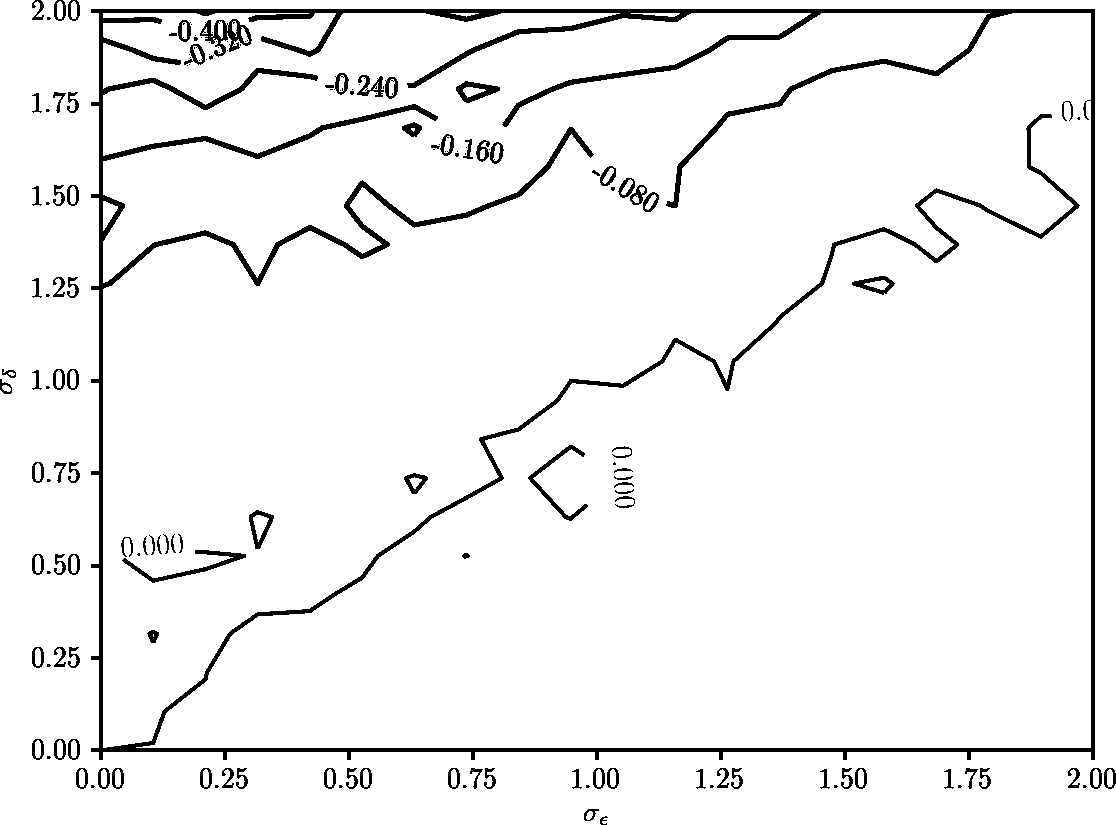
\includegraphics[width=135mm]{fig/linear/param/beta-0,125_param.png}
    \caption{\( \beta = 0{,}125 \)}
  \end{subfigure}

  \vspace{2\baselineskip}
  \begin{subfigure}[b]{\linewidth}
    \centering
    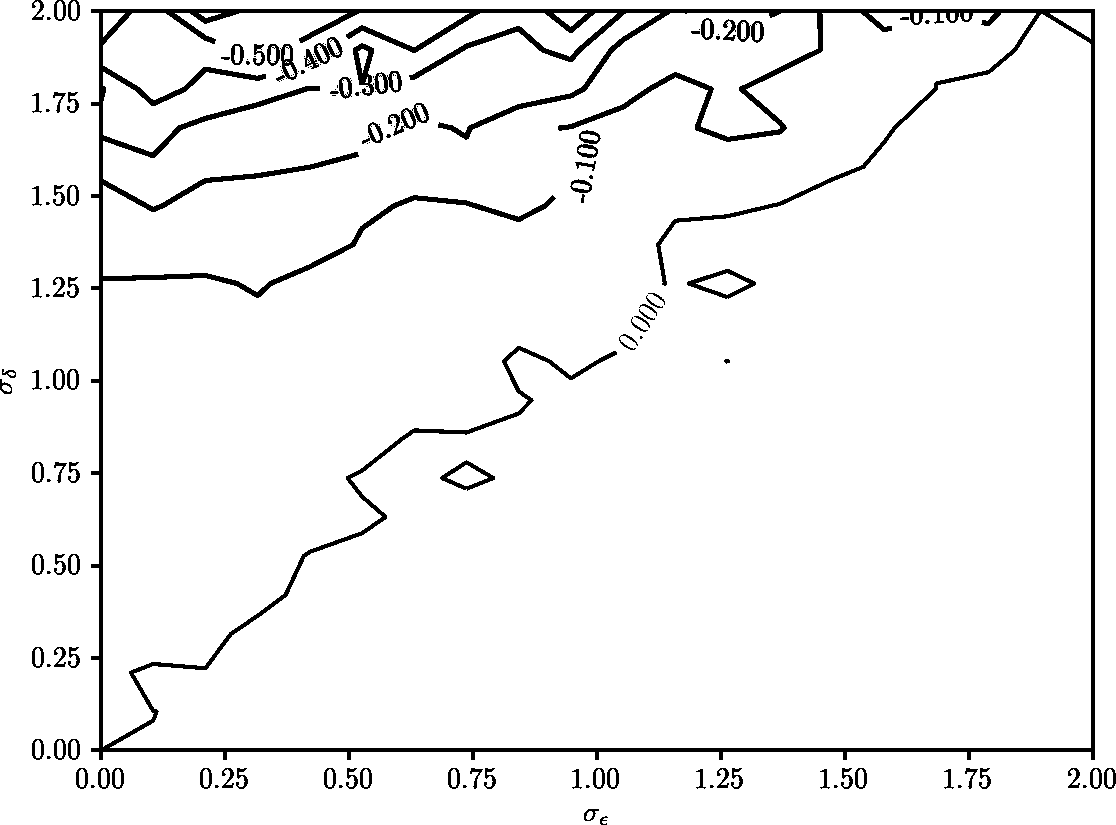
\includegraphics[width=135mm]{fig/linear/param/beta-0,2_param.png}
    \caption{\( \beta = 0{,}2 \)}
  \end{subfigure}

  \vspace{\baselineskip}
  \caption{%
    Сравнительная точность оценивания параметров линейных \\
    моделей с малыми коэффициентами усиления
  }\label{fig:comparison_linear_params_beta-small}
\end{figure}

На рисунке~\ref{fig:comparison_linear_params_beta-0,5}
представлены линии равного уровня зависимости \( d(\sigma_{\varepsilon_x}, \sigma_{\varepsilon_y}) \)
при \( \beta = 0{,}5 \).
Поскольку при \( \sigma_{\varepsilon_y} > \sigma_{\varepsilon_x} \)
значение \( d \) отрицательно (\( d \in ( -1, 0 ] \)),
можно сделать вывод, что МНК даёт более точные оценки параметров, чем МСА.
В отличие от предыдущего случая,
при \( \sigma_{\varepsilon_y} \le \sigma_{\varepsilon_x} \)
значение \( d \) положительно (\( d \in [0, 0{,}5 ) \)),
поэтому МСА дает немного более точные оценки параметров, чем МНК.

\begin{figure}[t]
  \centering
  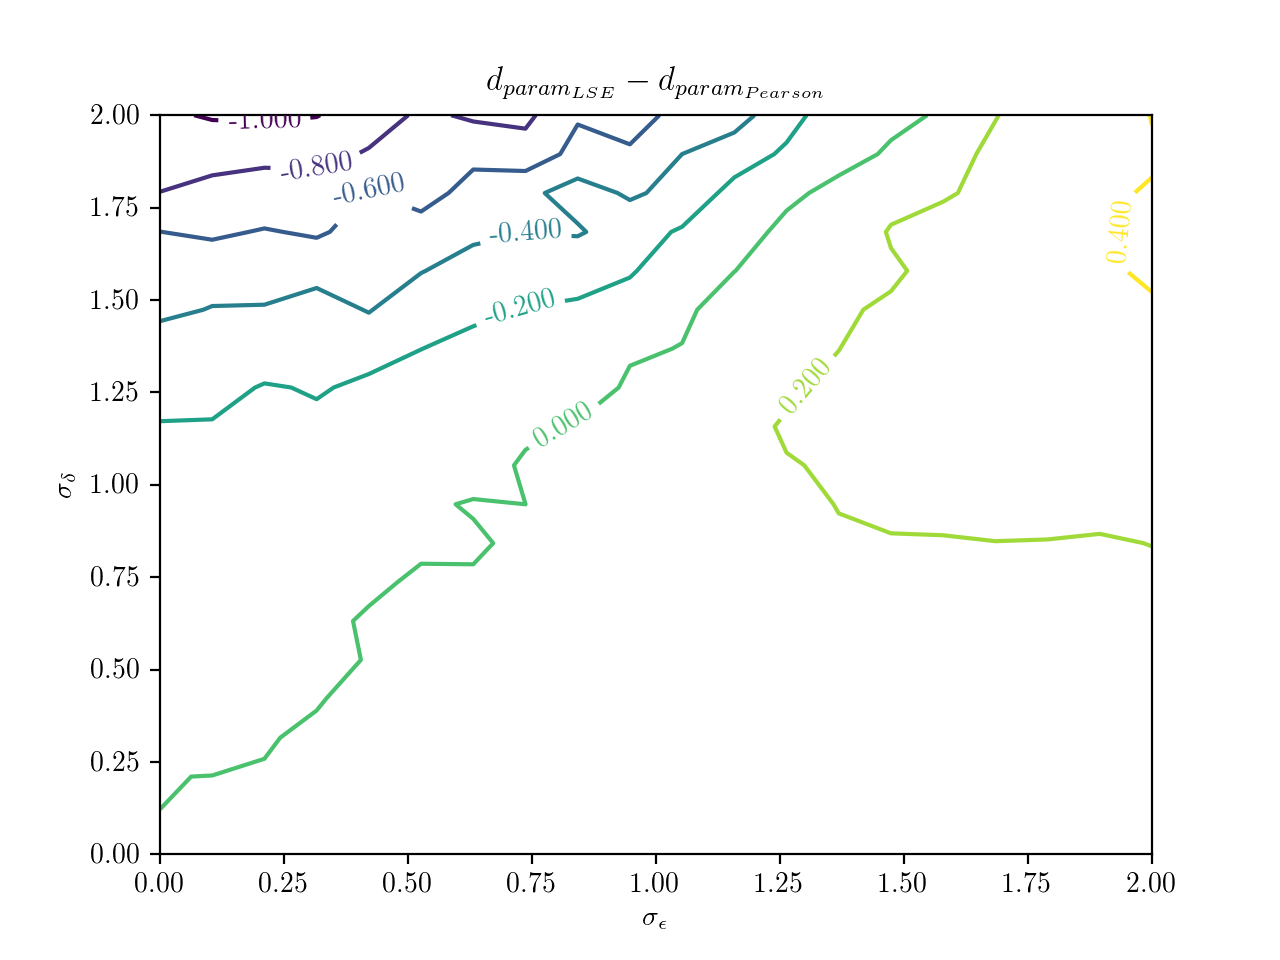
\includegraphics[width=135mm]{fig/linear/param/beta-0,5_param.png}
  \caption{%
    Сравнительная точность оценивания параметров линейной \\
    модели с коэффициентом усиления \( \beta = 0{,}5 \)
  }\label{fig:comparison_linear_params_beta-0,5}
\end{figure}

\pagebreak
На рисунке~\ref{fig:comparison_linear_params_beta-1}
представлены линии равного уровня функции \( d(\sigma_{\varepsilon_x}, \sigma_{\varepsilon_y}) \)
при \( \beta = -1 \) и \( \beta = 1 \).
Поскольу эти {\color{red} графики} практически совпадают, можно утверждать, что точность рассматриваемых
методов зависит лишь от абсолютного значения коэффициента усиления \( \beta \) и
не зависит от его знака.
Данное утверждение остается справедливым во всех рассмотренных случаях.

Красными точками отмечены пары значений с.~к.~о. ошибок наблюдений, при которых \( d = 0 \).
Эти значения были аппроксимированы с помощью МСА линейными функциями,
представленными на рисунке прямыми красного цвета.
Прямые синего цвета соответствует приближенной зависимости~\eqref{eq:rule_linear_param}.

Нетрудно заметить, что на рассматриваемых рисунках линии равного уровня функции
\( d(\sigma_{\varepsilon_x}, \sigma_{\varepsilon_y}) \)
симметричны относительно линии нулевого уровня данной функции.

При \( \sigma_{\varepsilon_y} > \sigma_{\varepsilon_x} \)
значение \( d \) отрицательно (\( d \in ( -1, 0 ] \)) ---
классическая линейная регрессия дает более точные оценки параметров, чем МСА.
При \( \sigma_{\varepsilon_y} \le \sigma_{\varepsilon_x} \)
значение \( d \) положительно (\( d \in [0, 1 ) \)),
поэтому метод симметричной аппроксимации дает более точные оценки параметров,
чем классическая линейная регрессия.

\begin{figure}[p]
  \begin{subfigure}[b]{\linewidth}
    \centering
    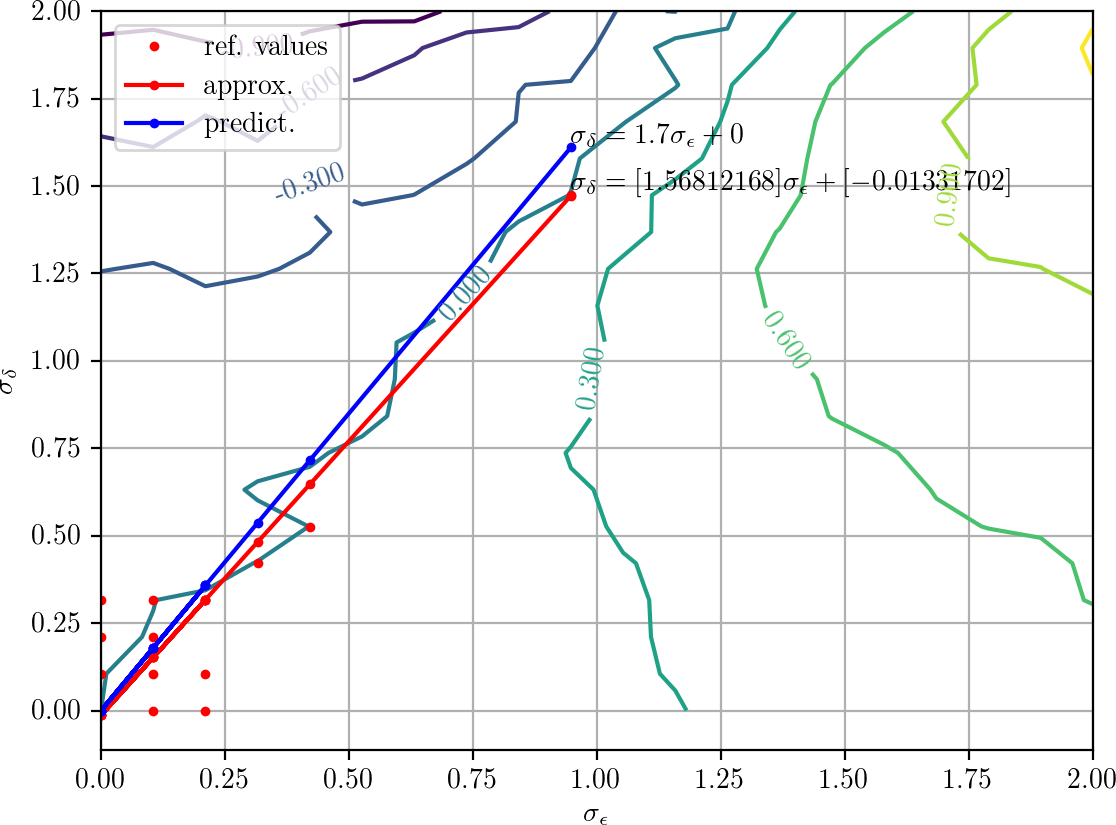
\includegraphics[width=135mm]{fig/linear/param/beta--1_param-accs-diff-approx}
    \caption{\( \beta = -1 \)}
  \end{subfigure}

  \vspace{2\baselineskip}
  \begin{subfigure}[b]{\linewidth}
    \centering
    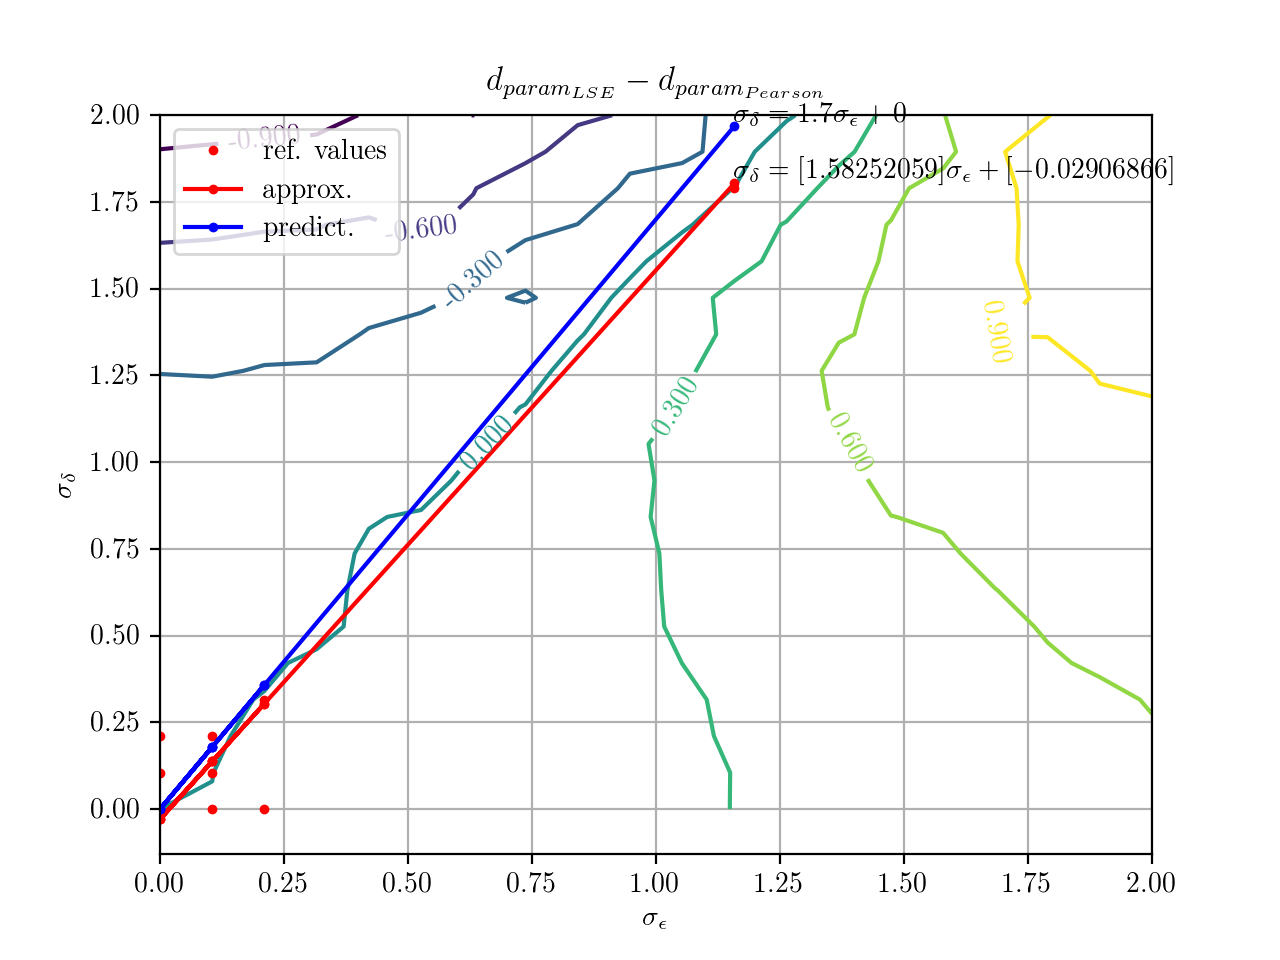
\includegraphics[width=135mm]{fig/linear/param/beta-1_param-accs-diff-approx}
    \caption{\( \beta = 1 \)}
  \end{subfigure}

  \vspace{\baselineskip}
  \caption{%
    Сравнительная точность оценивания параметров линейных \\
    моделей с единичным коэффициентом усиления
  }\label{fig:comparison_linear_params_beta-1}
\end{figure}

\pagebreak
На рисунке~\ref{fig:comparison_linear_params_beta-2}
представлены линии равного уровня функции \( d(\sigma_{\varepsilon_x}, \sigma_{\varepsilon_y}) \)
при \( \beta = 2 \).
Поскольку при \( \sigma_{\varepsilon_y} > 2 \sigma_{\varepsilon_x} \)
значение \( d \) невелико по модулю и отрицательно (\( d \in ( -0{,}5, 0 ] \)),
МНК дает более немного точные оценки параметров, чем МСА.
При \( \sigma_{\varepsilon_y} \le 2\sigma_{\varepsilon_x} \)
значение \( d \) положительно (\( d \in [0, 2{,}5 ) \)),
поэтому МСА дает более точные оценки параметров, чем МНК.

\begin{figure}[h]
  \centering
  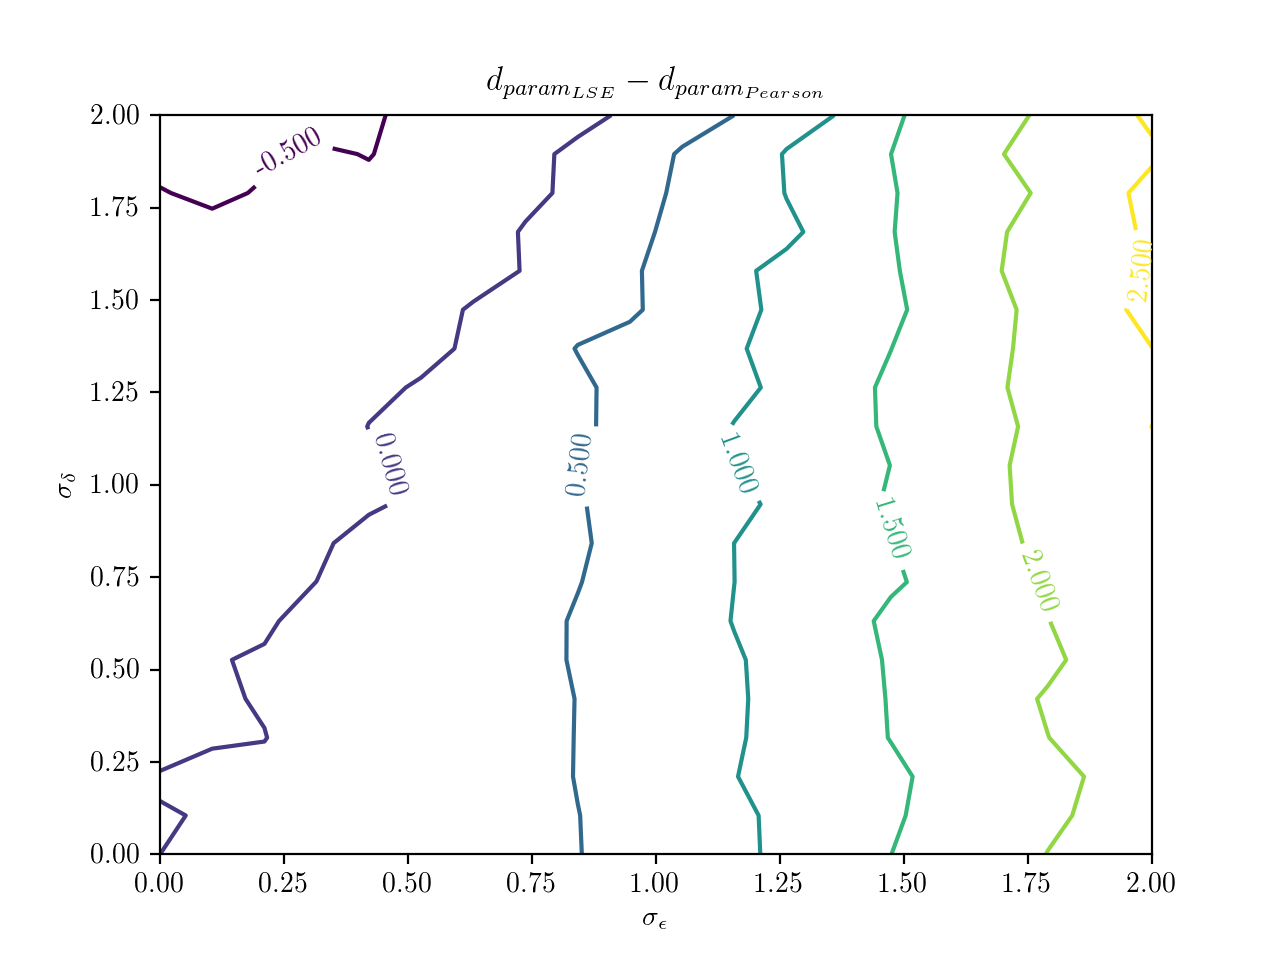
\includegraphics[width=135mm]{fig/linear/param/beta-2_param.png}
  \caption{%
    Сравнительная точность оценивания параметров линейной \\
    модели с коэффициентом усиления \( \beta = 2 \)
  }\label{fig:comparison_linear_params_beta-2}
\end{figure}

Следует отметить, что в рассмотренном случае область предпочтительного использования
МСА для оценивания точности параметров значительно больше, чем у МНК,
а при \( \sigma_{\varepsilon_x} \gg \sigma_{\varepsilon_y} \) точность МСА значительно выше.

Данная тенденция усиливается при больших коэффициентах усиления модели
(рисунок~\ref{fig:comparison_linear_params_beta-big}).
При \( \sigma_{\varepsilon_y} > 8\sigma_{\varepsilon_x} \)
значение величины \( d \) невелико по модулю и отрицательно: \( d \in ( -0{,}5, 0 ] \),
МНК дает немного более точные оценки параметров, чем МСА.
При увеличении \( \sigma_{\varepsilon_y} \) относительно \( \sigma_{\varepsilon_x} \) значение
\( d \) быстро нарастает, что свидетельствует о том,
что при данных условиях МСА дает значительно более точные оценки параметров, чем МНК.

\begin{figure}[p]
  \begin{subfigure}[b]{\linewidth}
    \centering
    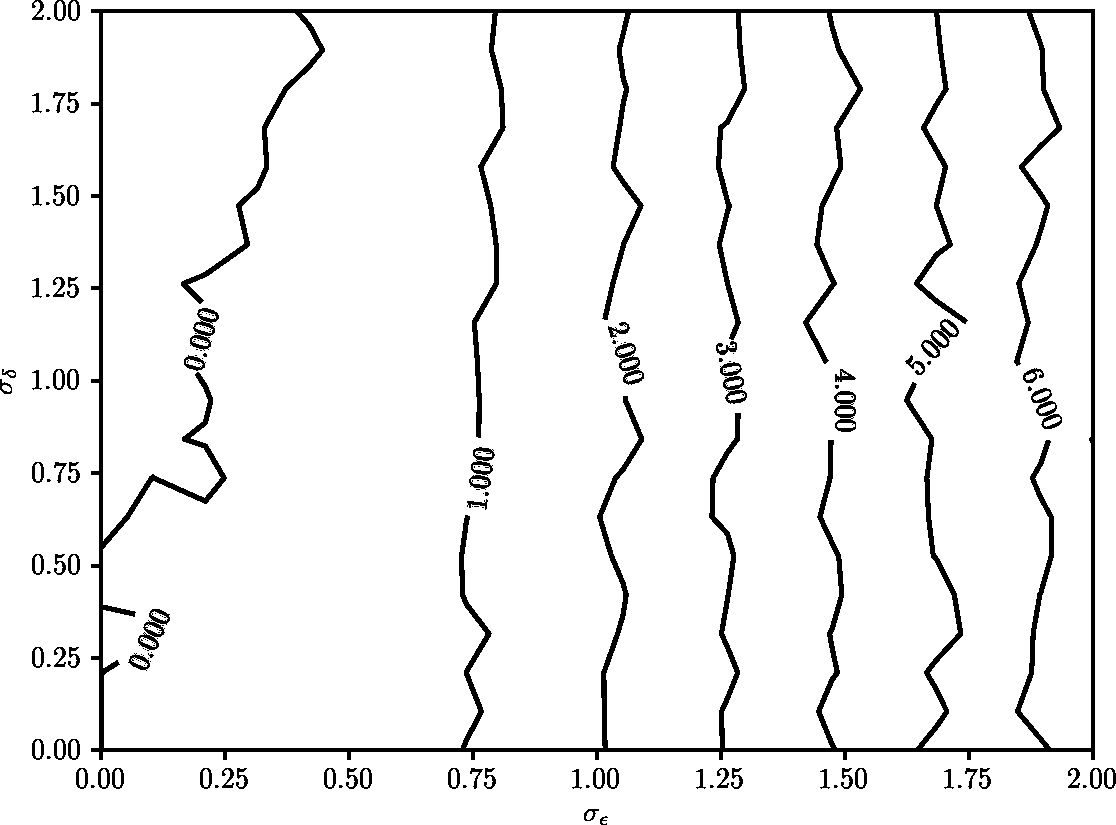
\includegraphics[width=135mm]{fig/linear/param/beta-5_param}
    \caption{\( \beta = 5 \)}
  \end{subfigure}

  \vspace{2\baselineskip}
  \begin{subfigure}[b]{\linewidth}
    \centering
    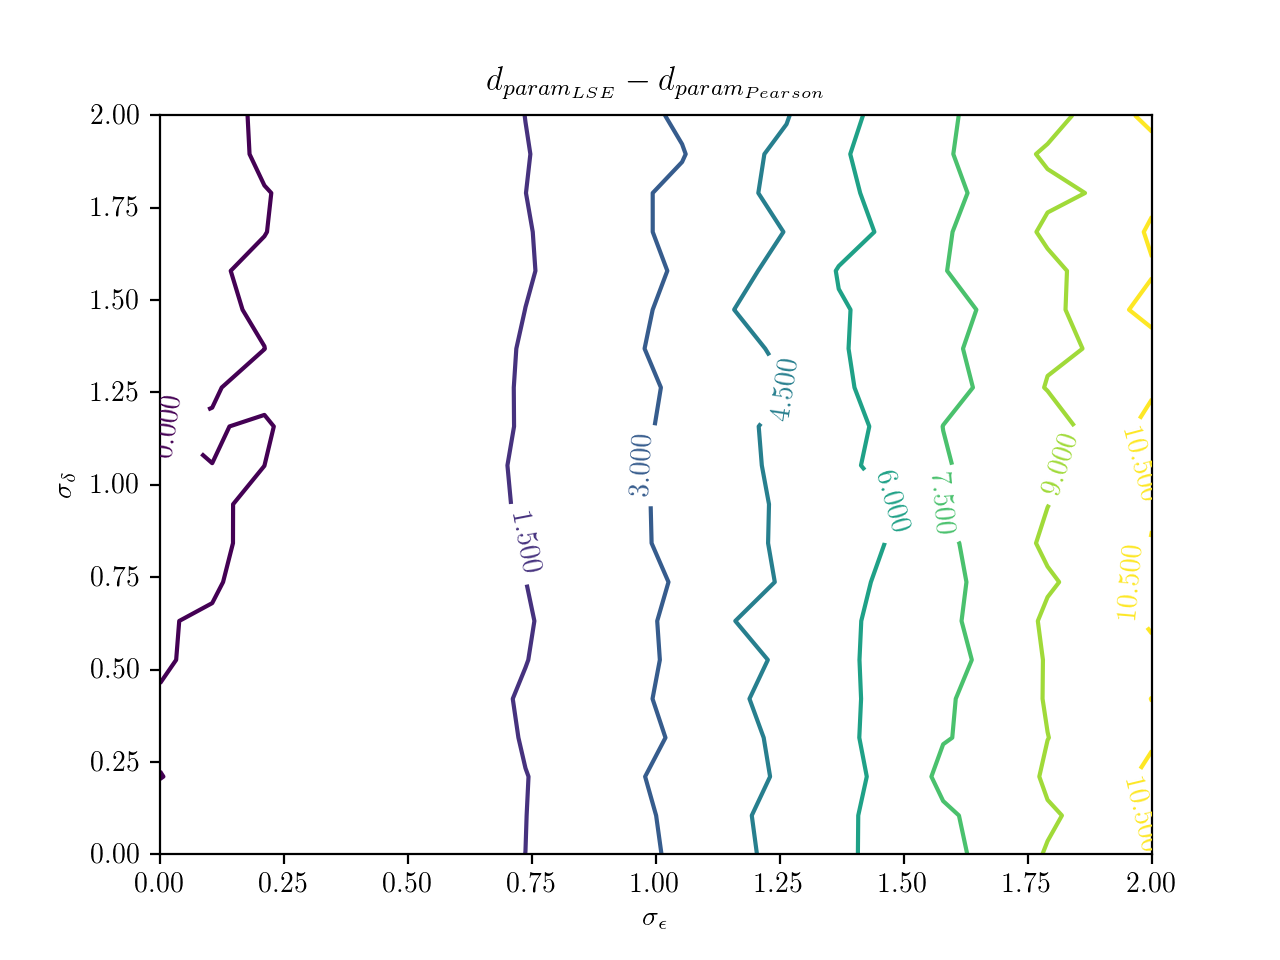
\includegraphics[width=135mm]{fig/linear/param/beta-8_param}
    \caption{\( \beta = 8 \)}
  \end{subfigure}

  \vspace{\baselineskip}
  \caption{%
    Сравнительная точность оценивания параметров линейных \\
    моделей с большими коэффициентами усиления
  }\label{fig:comparison_linear_params_beta-big}
\end{figure}

\pagebreak
На основании изложенного можно сделать следуюшие выводы:
\begin{enumerate}
\item Точность оценивания параметров не зависит от фактического значение постоянной
  составляющей \( \alpha \).
\item Точность оценивания параметров зависит от абсолютного значения коэффициента усиления системы и
  значений с.~к.~о. ошибок измерений входных и выходных переменных.
  С ростом величины коэффициента усиления и с.~к.~о. ошибок наблюдений
  входных переменных метод симметричной аппроксимации дает более точные оценки,
  чем метод наименьших квадратов.
\item При больших значениях коэффициента усиления \( |\beta| > 2 \)
  точность симметричного оценивания значительно превосходит
  точность классического подхода.
\item Для того, чтобы решить, какой метод предпочтительно использовать для оценивания параметров
  линейной стохастической системы второго типа,
  предлагается использовать следующее эмпирическое правило: {\color{red} обосновать}
  <<Если условие
  \begin{equation}
    \sigma_{\varepsilon_y} < (0{,}7 + |\beta|) \sigma_{\varepsilon_x}
    \label{eq:rule_linear_param}
  \end{equation}
  выполняется, то метод симметричной аппроксимации оценивает параметры системы
  второго типа более точно, чем классическая линейная регрессия>>.
\end{enumerate}

\pagebreak
\subsection{Точность прогнозирования наблюдений выхода}

Было выполнено сравнение точности прогнозирования наблюдений выхода по
наблюдениям входа системы~\eqref{eq:linear_model_scalar} на основании оценкок параметров,
полученными методом наименьших квадратов и методом симметричной аппроксимации,
в зависимости от c.~к.~о. ошибок наблюдений \( \sigma_{\varepsilon_x}, \sigma_{\varepsilon_y} \).

В качестве величины, характеризующей точность прогнозирования,
использовалась разность средних Евклидовых расстояний между наблюдениями выхода модели и
их оценками, полученными МНК и МСА:
\begin{equation*}
  \begin{aligned}
    d &= d_{\text{МНК}} - d_{\text{МСА}}, \\
    d_{\text{МНК}} &= \frac{1}{k} \sum_{j=1}^k \sqrt{ \sum_{i=1}^n (\hat{\alpha}_{\text{МНК}_j} + \hat{\beta}_{\text{МНК}_j} x_{ij} - y_{ij})^2}, \\
    d_{\text{МСА}} &= \frac{1}{k} \sum_{j=1}^k \sqrt{ \sum_{i=1}^n (\hat{\alpha}_{\text{МСА}_j} + \hat{\beta}_{\text{МСА}_j} x_{ij} - y_{ij})^2},
    \end{aligned}
  \end{equation*}
где \( k \) --- число оценок.

Расчеты расстояний \( d \) производились в узлах сетки значений
\( \sigma_{\varepsilon_x}, \sigma_{\varepsilon_y} \) в прямоугольнике
\( [0, 2] \times [0, 2] \) с шагом 0{,}1.
В каждом узле сетки вычислялось сто оценок (\( k = 100 \)).
Для получения каждой оценки \( \hat{\alpha}, \hat{\beta} \) использовались результаты
ста наблюдений \( ( x_i, y_i ), i = \overline{1, n}, n = 100 \).

{\color{red}
Таким образом, при \( d > 0 \) точность оценивания параметров модели с помощью МСА
превосходит точность МНК, а при \( d < 0 \) МНК-оценки являются более точными.
При \( d = 0 \) оба метода дают оценки одинаковой точности.
}

На рисунке~\ref{fig:comparison_linear_predict} представлены линии равного уровня
зависимости \( d(\sigma_{\varepsilon_x}, \sigma_{\varepsilon_y}) \) при различных
значениях коэффициента усиления модели \( \beta \).
Нетрудно убедиться, что классический метод наименьших квадратов дает более точные оценки
наблюдаений выхода по наблюдениям входа системы, чем метод симметричной аппроксимации
во всем рассмотренном диапазоне значений коэффициента усиления и с.~к.~о. ошибок наблюдений.

\begin{figure}[h]
  \begin{subfigure}[b]{\linewidth}
    \centering
    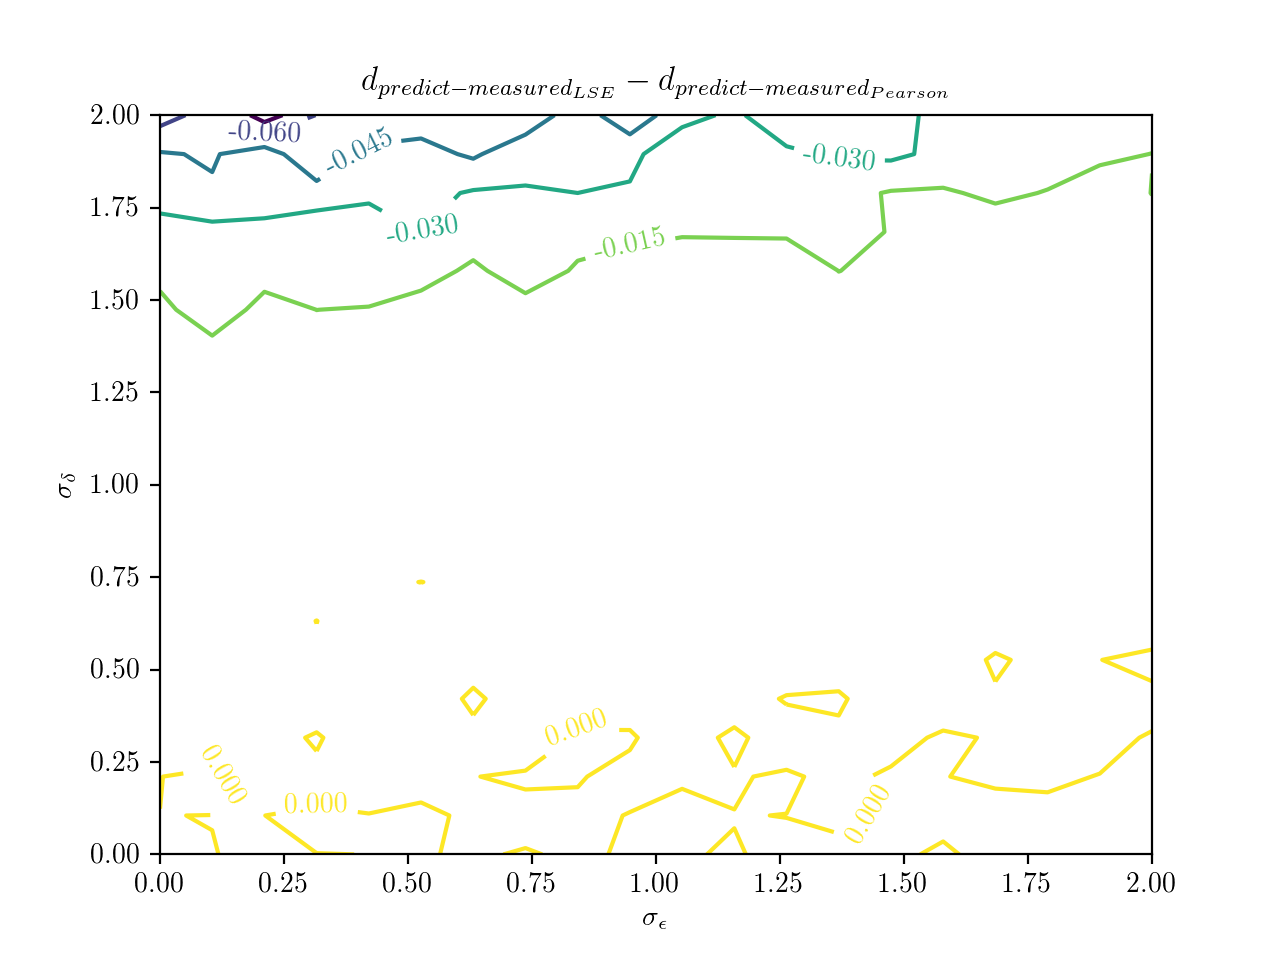
\includegraphics[width=135mm]{fig/linear/predict/beta-0,2_predict-measured.png}
    \caption{\( \beta = 0{,}2 \)}
  \end{subfigure}

  \vspace{2\baselineskip}
  \begin{subfigure}[b]{\linewidth}
    \centering
    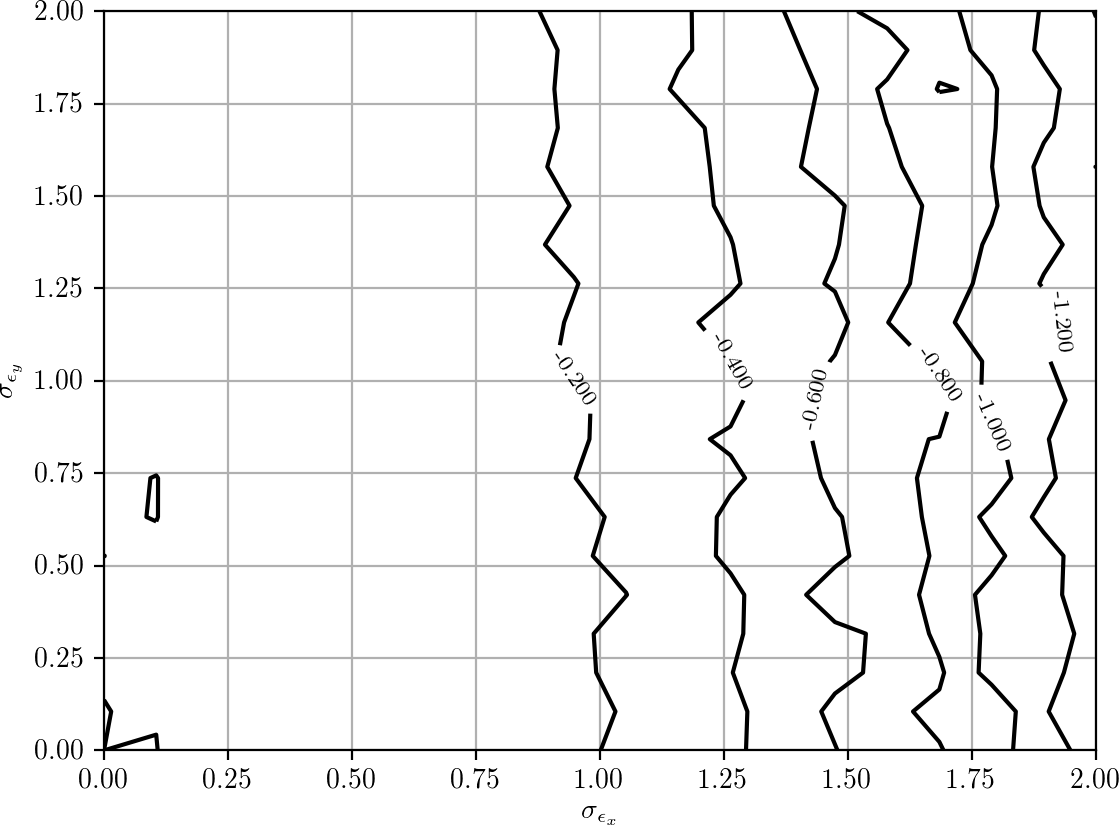
\includegraphics[width=135mm]{fig/linear/predict/beta-5_predict-measured.png}
    \caption{\( \beta = 5 \)}
  \end{subfigure}

  \vspace{\baselineskip}
  \caption{%
    Сравнительная точность прогнозирования \\
    наблюдений выхода линейной модели
  }\label{fig:comparison_linear_predict}
\end{figure}

\section{Выводы}

Выводы по главе 2.